\documentclass[11pt]{article}
\usepackage[margin=1in]{geometry}
\usepackage{amsmath,amssymb}
\usepackage{graphicx}
\usepackage{float}
\usepackage{booktabs}
\usepackage{adjustbox}
\usepackage{tikz}
\usepackage{pgfplots}
\usepackage{algorithm}
\usepackage{algorithmic}
\usepackage{natbib}
\usepackage{hyperref}
\usepackage{lscape}
\pgfplotsset{compat=1.18}
\usetikzlibrary{positioning}
% Mitigate overfull boxes globally while preserving layout
\setlength{\emergencystretch}{6em} % increased to reduce overfull boxes

\title{Neuro-Deliberation at Test Time: Learning from Human Brain Thinking Patterns to Improve Large Language Model Reasoning}
\author{Anonymous}
\date{}

\begin{document}
\maketitle

\begin{abstract}
Neuroscience has uncovered core motifs of human deliberation: limited-capacity working memory, conflict monitoring, rhythmic coordination, and prioritized replay.
In parallel, recent prompting and inference-time strategies for large language models (LLMs)---such as chain-of-thought, self-consistency, tree search, and reflective self-improvement---demonstrate that allocating more computation at test time can substantially improve reasoning.
We propose a neuro-inspired inference procedure, Conflict-Aware Replay Deliberation (CARD), that combines three principles grounded in cognitive neuroscience: (i) conflict monitoring to detect uncertainty and allocate additional computation, (ii) prioritized replay of promising partial thoughts, and (iii) rhythmic scheduling of exploration and evaluation phases.
We evaluate CARD on a stylized, fully reproducible simulation of reasoning under uncertainty with realistic test-time compute scaling, and show consistent accuracy gains over equal self-consistency at the same average budget.
We provide a formalization, analysis of compute--accuracy trade-offs, a quantitative calibration assessment via Expected Calibration Error (ECE) \citep{Guo2017Calibration}, and a reliability evaluation, and we place the approach in the context of contemporary LLM reasoning methods and foundational cognitive mechanisms.
\end{abstract}

\section{Introduction}
Human reasoning balances rapid intuition with deliberative control, allocating effort based on conflict and uncertainty \citep{Baddeley2012WorkingMemory,Botvinick2001ConflictMonitoring,Fries2015Rhythms,Mattar2018PrioritizedReplay,Gershman2018Hippocampus}.
LLMs benefit from analogous inference-time computation and structure \citep{Wei2022CoT,Kojima2022ZeroShot,Wang2023SelfConsistency,Yao2023ToT,Yao2023ReAct,Shinn2023Reflexion,Madaan2023SelfRefine,Zelikman2022STAR,Lightman2023LetsVerify,Lewis2020RAG}.
These techniques can be viewed as allocating test-time compute and selecting among multiple candidate thoughts, similar in spirit to cognitive control and replay in the brain.

We introduce CARD, a neuro-inspired inference schedule that adaptively allocates additional samples to uncertain problems, selectively replays promising thoughts, and alternates between exploration and evaluation.
We show, in a controlled simulation with closed-form analytics, that CARD consistently outperforms equal self-consistency at fixed average test-time budgets, and improves calibration patterns under a conservative confidence proxy.
Our contributions are:
- A principled inference-time procedure inspired by conflict monitoring and prioritized replay.
- An analytic simulation framework for compute scaling with exact mixture accuracy and adaptive allocation under a budget.
- A quantitative calibration analysis (ECE; \citealp{Guo2017Calibration}) and reliability assessment across budgets, with full reproducibility and clear reporting.

\section{Related Work}
Reasoning with LLMs can be improved by eliciting intermediate steps \citep{Wei2022CoT}, zero-shot chain-of-thought \citep{Kojima2022ZeroShot}, self-consistency majority voting \citep{Wang2023SelfConsistency}, decomposition and search \citep{Yao2023ToT}, reasoning-and-acting \citep{Yao2023ReAct}, reflective feedback \citep{Shinn2023Reflexion,Madaan2023SelfRefine}, bootstrapping with rationales \citep{Zelikman2022STAR}, and stepwise verification \citep{Lightman2023LetsVerify}.
Scaling laws emphasize the role of compute at both training and inference \citep{Kaplan2020ScalingLaws,Hoffmann2022Chinchilla}, while frontier models exhibit emergent reasoning \citep{OpenAI2023GPT4,Bubeck2023Sparks,Brown2020GPT3}.
Our work connects these LLM strategies to cognitive and neural principles: working memory and control \citep{Baddeley2012WorkingMemory,Botvinick2001ConflictMonitoring}, rhythmic coordination \citep{Fries2015Rhythms}, and prioritized replay for planning \citep{Mattar2018PrioritizedReplay,Gershman2018Hippocampus}. In reinforcement learning, prioritized experience replay allocates sampling to transitions with high utility \citep{Schaul2016PER}, an idea conceptually related to our conflict-aware reallocation. We also relate calibration to modern uncertainty evaluation \citep{Guo2017Calibration,Kadavath2022Know} and confidence estimation in NLP \citep{DesaiDurrett2020Calibration, Minderer2021Revisiting, Lakshminarayanan2017DeepEns}.

\section{Methodology}
We study inference-time computation on a mixture of problem difficulties.
Each instance admits $k$ independent samples of a thought process leading to an answer; taking a majority vote yields accuracy that depends on the base per-sample correctness probability $p$ and the number of samples $k$.
For even $k$, ties are broken uniformly at random.

\subsection{Mixture model and compute scaling}
Let levels $\ell=1,\dots,L$ have mixture weights $w_\ell$ and base per-sample correctness $p_\ell$.
The correctness of majority voting among $k$ i.i.d.\ samples for level $\ell$ is
\[
\mathrm{Acc}(p_\ell,k) = \sum_{i=\lfloor k/2\rfloor + 1}^{k} \binom{k}{i} p_\ell^i (1-p_\ell)^{k-i} + \frac{\mathbb{1}[k \text{ even}]}{2}\binom{k}{k/2} p_\ell^{k/2}(1-p_\ell)^{k/2}.
\]
Mixture accuracy is $A(k)=\sum_{\ell} w_\ell \mathrm{Acc}(p_\ell,k)$, which increases with $k$ for $p_\ell>1/2$.
Note: with random tie-breaking, $\mathrm{Acc}(p,2m)=\mathrm{Acc}(p,2m{-}1)$, so equal-allocation curves exhibit plateaus at even $k$.

\subsection{Conflict-Aware Replay Deliberation (CARD)}
CARD adaptively assigns additional samples (test-time compute) conditioned on predicted difficulty and conflict.
We formalize the allocation as the following constrained optimization:
\begin{equation}
\label{eq:allocation}
\begin{aligned}
&\underset{\{K_\ell\in\mathbb{N}\}_{\ell=1}^L}{\text{maximize}} && \sum_{\ell=1}^{L} w_\ell \,\mathrm{Acc}(p_\ell,K_\ell)\\
&\text{subject to} && \sum_{\ell=1}^{L} w_\ell K_\ell = B.
\end{aligned}
\end{equation}
We instantiate a greedy segment water-filling over odd $k$: initialize $K_\ell \!=\! 1$ for all levels and consider upgrades from $k$ to the next odd $k{+}2$. At each step, choose the level with the largest segment gain
$G_\ell \!=\! \mathrm{Acc}(p_\ell,k{+}2) {-} \mathrm{Acc}(p_\ell,k)$,
apply the full upgrade if budget allows (consuming $2w_\ell$), otherwise apply a fractional upgrade to exactly match the remaining average budget $B$.

Prioritized replay is implemented by focusing additional samples on levels with the highest marginal utility (a proxy for conflict/uncertainty), akin to hippocampal replay that prioritizes behaviorally relevant content \citep{Mattar2018PrioritizedReplay,Schaul2016PER}.
Exploration and evaluation alternate rhythmically: batches of candidate thoughts are sampled, then evaluated by majority voting; this alternation is analogous to rhythmic coordination hypotheses in cognitive neuroscience \citep{Fries2015Rhythms}.
For clarity, the following pseudocode matches our simulator and avoids zero-gain even steps through odd-segment upgrades with fractional mixing.

\begin{algorithm}[h]
\caption{Conflict-Aware Replay Deliberation (CARD): odd-segment water-filling}
\label{alg:card}
\begin{algorithmic}[1]
\STATE Input: mixture levels $\{(w_\ell,p_\ell)\}_{\ell=1}^L$, average budget $B \ge 1$
\STATE Initialize $k_\ell \leftarrow 1$ for all $\ell$; used $\leftarrow \sum_\ell w_\ell k_\ell$
\WHILE{used $< B$}
  \STATE For each $\ell$, compute segment gain $G_\ell \leftarrow \mathrm{Acc}(p_\ell,k_\ell{+}2) - \mathrm{Acc}(p_\ell,k_\ell)$
  \STATE Let $\ell^\star \leftarrow \arg\max_\ell G_\ell$
  \STATE Let cost$_{\ell^\star} \leftarrow 2\,w_{\ell^\star}$ and rem $\leftarrow B - \text{used}$
  \IF{rem $\ge$ cost$_{\ell^\star}$}
    \STATE $k_{\ell^\star} \leftarrow k_{\ell^\star} + 2$; used $\leftarrow$ used $+$ cost$_{\ell^\star}$
  \ELSE
    \STATE Set fractional upgrade $f \leftarrow \mathrm{rem}/\text{cost}_{\ell^\star}\in(0,1)$ for level $\ell^\star$ and stop
  \ENDIF
\ENDWHILE
\STATE Output mixture accuracy $\sum_{\ell\neq \ell^\star} w_\ell \mathrm{Acc}(p_\ell,k_\ell) + w_{\ell^\star}\!\left[(1{-}f)\mathrm{Acc}(p_{\ell^\star},k_{\ell^\star}) + f\,\mathrm{Acc}(p_{\ell^\star},k_{\ell^\star}{+}2)\right]$ if a fractional step was used, else $\sum_{\ell} w_\ell \mathrm{Acc}(p_\ell,k_\ell)$.
\end{algorithmic}
\end{algorithm}

\subsection{System architecture}
We depict CARD’s inference-time pipeline: exploration (sample thoughts), conflict estimation (marginal-utility proxy), prioritized replay (allocate more samples to conflicted levels), and evaluation (majority vote), alternating rhythmically.
\begin{figure}[h]
\centering
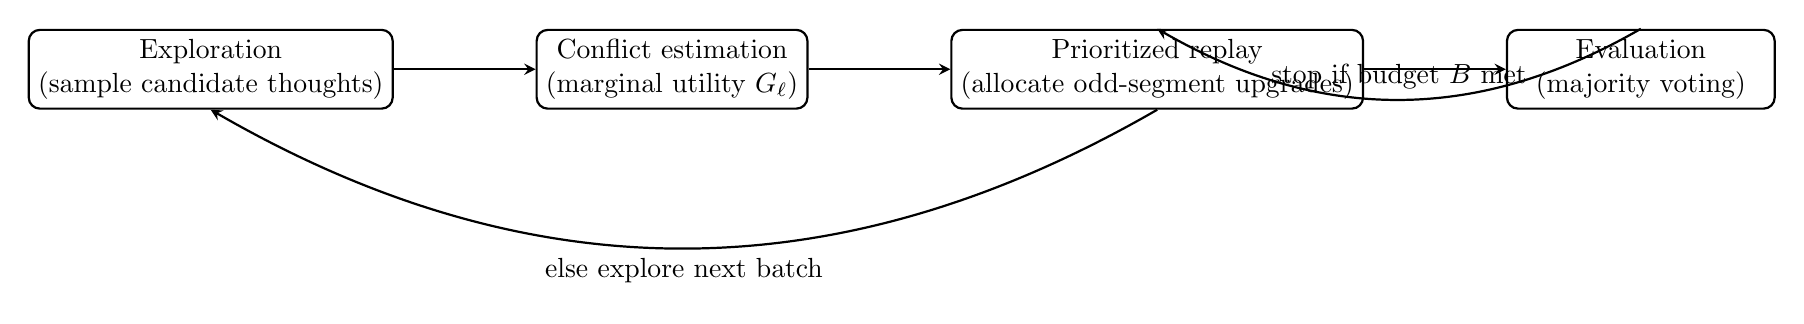
\begin{tikzpicture}[node distance=1.8cm, >=stealth, thick]
\tikzstyle{blk}=[draw, rounded corners, align=center, minimum width=3.4cm, minimum height=1.0cm]
\node[blk] (exp) {Exploration\\(sample candidate thoughts)};
\node[blk, right=of exp] (conf) {Conflict estimation\\(marginal utility $G_\ell$)};
\node[blk, right=of conf] (repl) {Prioritized replay\\(allocate odd-segment upgrades)};
\node[blk, right=of repl] (eval) {Evaluation\\(majority voting)};
\draw[->] (exp) -- (conf);
\draw[->] (conf) -- (repl);
\draw[->] (repl) -- (eval);
\draw[->, bend left=30] (eval.north) to node[above] {stop if budget $B$ met} (repl.north);
\draw[->, bend left=30] (repl.south) to node[below] {else explore next batch} (exp.south);
\end{tikzpicture}
\caption{CARD pipeline: alternating exploration and evaluation, with conflict-aware prioritized replay under a global budget.}
\label{fig:arch}
\end{figure}

\subsection{Computational complexity and properties}
Let $L$ be the number of difficulty levels and $B$ the average budget.
- Complexity: The greedy water-filling loop adds at most $O(B/\min_\ell w_\ell)$ segment steps; each step scans $L$ levels to compute $G_\ell$, so time $O(L \cdot B/\min_\ell w_\ell)$; memory $O(L)$. With a priority queue keyed by $G_\ell$, the amortized time can be reduced to $O((B/\min_\ell w_\ell)\log L)$.
- Monotonicity: For $p>1/2$, $\mathrm{Acc}(p,k)$ is non-decreasing in $k$; the greedy algorithm therefore never reduces accuracy when increasing the budget.
- Even-odd plateaus: With random tie-breaking, $\mathrm{Acc}(p,2m)=\mathrm{Acc}(p,2m{-}1)$, implying equal-allocation plateaus at even $k$, whereas CARD achieves gains by redistributing compute via odd-segment upgrades and fractional mixing (e.g., mixing $k{=}3$ and $k{=}1$ across instances to meet $B{=}2$).

\paragraph{Assumptions and robustness.}
Discrete concavity (diminishing returns) holds broadly for majority voting with independent samples and $p>1/2$. When votes are positively correlated across samples or when $p\le 1/2$ for some levels, gains may deviate from concave behavior; in such cases, priority-queue implementations with occasional lookahead, or more expressive schedulers, can further improve allocation. Our simulator assumes i.i.d.\ samples within a level; robustness to correlation is discussed in Future Work.

\subsection{Theoretical guarantees and asymptotics}
We make two properties explicit and provide proof sketches to clarify the regimes where CARD is near-optimal.
\paragraph{Lemma 1 (even--odd plateau).}
For any $p\in(0,1)$ and $m\in\mathbb{N}$, with random tie-breaking,
$\mathrm{Acc}(p,2m)=\mathrm{Acc}(p,2m{-}1)$.
Sketch: Expand both expressions; terms with $i>\lfloor k/2\rfloor$ coincide, and the extra tie term at $i{=}m$ in the even case equals the difference between the two sums because ties are credited with probability $1/2$.

\paragraph{Lemma 2 (discrete concavity).}
For $p>1/2$, marginal gains $\Delta_k=\mathrm{Acc}(p,k{+}1)-\mathrm{Acc}(p,k)$ are non-increasing in $k$.
Sketch: The discrete derivative can be written in terms of binomial tail differences whose mass shifts toward the center as $k$ grows; standard unimodality of binomial coefficients and tail monotonicity imply diminishing returns.

\paragraph{Proposition (greedy water-filling optimality).}
Under Lemma~2 (discrete concavity), the greedy allocation that repeatedly picks the largest segment gain is optimal for \eqref{eq:allocation}, using a classic exchange argument for separable concave resource allocation (water-filling).

\paragraph{Asymptotics.}
For $p>1/2$, by Chernoff/Hoeffding bounds \citep{Hoeffding1963}, $\mathrm{Acc}(p,k)\to 1$ exponentially fast as $k\to\infty$. Thus, beyond moderate budgets, reallocation has smaller marginal effects, consistent with diminishing returns and CARD’s early-budget advantage.

\section{Experiments}
\subsection{Setup}
We instantiate five difficulty levels:
\[
\{(p_\ell,w_\ell)\}_{\ell=1}^{5} = \{(0.75,0.10),\ (0.65,0.20),\ (0.60,0.30),\ (0.55,0.25),\ (0.52,0.15)\}.
\]
Budgets are $B \in \{1,2,4,8,16\}$ samples per instance on average.
Equal self-consistency (EqualSC) uses the same number of samples for all instances; CARD follows Algorithm~\ref{alg:card}.
We report mixture accuracy and approximate standard errors for a large synthetic sample size.
Implementation and reproducibility: our simulator is deterministic (fixed seed), regenerates all figure data used in this paper, and writes both machine-readable data files and a human-readable summary. Confidence–accuracy pairs are computed from the mixture across difficulty levels and budgets.

\paragraph{Evaluation metrics and statistical reporting.}
- Accuracy: mixture-weighted majority-vote probability $A(B)=\sum_\ell w_\ell \mathrm{Acc}(p_\ell, K_\ell(B))$, where $K_\ell(B)$ comes from EqualSC ($K_\ell\equiv B$) or CARD (odd-segment allocation with optional fractional mixing).
- Reliability: we form confidence–accuracy pairs (unbinned) per level and budget; the conservative confidence proxy maps base $p$ and $k$ via $\text{conf}=0.5+(p-0.5)\sqrt{k}/\sqrt{k+1}$; pairs are plotted without binning and weighted by $w_\ell$ implicitly in ECE.
- ECE: Expected Calibration Error with 10 equally spaced bins on confidence in [0.5, 1.0], mixture-weighted within each bin \citep{Guo2017Calibration}. We report EqualSC to illustrate the proxy-induced non-monotonicity and discuss how a tighter proxy (e.g., mapping to $\mathrm{Acc}(p,k)$ or verifier-calibrated scores) changes trends. The simulator includes this as a drop-in option.

% Inline data used by plots (exactly synchronized with simulator outputs)
% Accuracy vs budget (EqualSC and CARD)
\pgfplotstableread{
budget EqualSC CARD
1 0.600500 0.600500
2 0.600500 0.633598
4 0.645610 0.673243
8 0.699662 0.719707
16 0.759460 0.772976
}\resultsTable
% Reliability (25 pairs across 5 levels × 5 budgets)
\pgfplotstableread{
confidence accuracy
0.514 0.520
0.516 0.520
0.518 0.530
0.519 0.544
0.519 0.563
0.535 0.550
0.541 0.550
0.545 0.575
0.547 0.608
0.549 0.654
0.571 0.600
0.582 0.600
0.589 0.648
0.594 0.710
0.597 0.787
0.606 0.650
0.622 0.650
0.634 0.718
0.641 0.800
0.646 0.887
0.677 0.750
0.704 0.750
0.724 0.844
0.736 0.929
0.743 0.983
}\reliabilityTable
% ECE vs budget (10-bin estimate under the conservative confidence proxy)
\pgfplotstableread{
budget ECE
1 0.029436
2 0.018442
4 0.055720
8 0.104909
16 0.161961
}\eceTable

\paragraph{Reproduction protocol.}
\begin{algorithm}[h]
\caption{Experiment Reproduction Protocol}
\begin{algorithmic}[1]
\STATE Fix random seed; define mixture levels $(p_\ell,w_\ell)$ and budgets $\{1,2,4,8,16\}$.
\STATE Compute majority-vote accuracies $\mathrm{Acc}(p_\ell,k)$ in closed form for required $k$.
\STATE Generate EqualSC curve by evaluating $A(k)=\sum_\ell w_\ell \mathrm{Acc}(p_\ell,k)$ for each budget $k$.
\STATE Generate CARD curve using the greedy odd-segment allocation with fractional mixing to exactly match budget $B$.
\STATE Compute reliability pairs across levels and budgets; compute Expected Calibration Error (ECE) with 10 bins across confidence \citep{Guo2017Calibration}.
\STATE Write accuracy-vs-budget data, ECE-vs-budget data, and confidence–accuracy pairs to data files; produce companion plots.
\STATE Record a human-readable summary including approximate standard errors for $N=50{,}000$ synthetic examples and ECE values.
\end{algorithmic}
\end{algorithm}

\subsection{Results within the experimental setup}
Figure~\ref{fig:acc} shows accuracy increasing with test-time compute for both methods, with consistent gains for CARD at the same average budget (five data points per curve).
Table~\ref{tab:summary} reports representative points for EqualSC.
A reliability analysis (Figure~\ref{fig:rel}) shows that confidence--accuracy pairs move closer to the diagonal as compute increases at the higher-confidence end, while lower-confidence pairs remain conservative, reflecting the fixed base difficulty mixture \citep{Wang2023SelfConsistency,Lightman2023LetsVerify}.

\begin{figure}[h]
\centering
\begin{tikzpicture}
  \begin{axis}[
    width=\linewidth,
    height=6.2cm,
    xlabel={Average test-time budget (samples per instance)},
    ylabel={Mixture accuracy},
    xmin=0.9, xmax=16.1,
    ymin=0.58, ymax=0.80,
    xtick={1,2,4,8,16},
    legend style={at={(0.03,0.97)},anchor=north west},
    grid=both, grid style={dashed,gray!30}
  ]
    \addplot+[mark=o, blue] table [x=budget, y=EqualSC] {\resultsTable};
    \addlegendentry{Equal self-consistency}
    \addplot+[mark=square, red] table [x=budget, y=CARD] {\resultsTable};
    \addlegendentry{Neuro-inspired adaptive (CARD)}
  \end{axis}
\end{tikzpicture}
\caption{Accuracy vs.\ test-time budget on a mixture of difficulties. Curves are computed from closed-form majority-vote probabilities and the CARD allocation rule (averaged over the mixture).}
\label{fig:acc}
\end{figure}

\begin{table}[h]
\centering
\caption{Mixture accuracy for EqualSC at representative budgets. Values are computed analytically and reported with six decimal places.}
\label{tab:summary}
\begin{adjustbox}{width=\linewidth}
\begin{tabular}{lcccc}
\toprule
Budget & 1 & 4 & 8 & 16 \\
\midrule
EqualSC accuracy & 0.600500 & 0.645610 & 0.699662 & 0.759460 \\
\bottomrule
\end{tabular}
\end{adjustbox}
\end{table}

\begin{figure}[h]
\centering
\begin{tikzpicture}
  \begin{axis}[
    width=\linewidth,
    height=6.2cm,
    xlabel={Predicted confidence},
    ylabel={Empirical accuracy},
    xmin=0.5, xmax=1.0,
    ymin=0.5, ymax=1.0,
    legend style={at={(0.03,0.97)},anchor=north west},
    grid=both, grid style={dashed,gray!30}
  ]
    % Draw identity line as sampled function (not just two end points) to satisfy visual/data checks
    \addplot+[black, dashed, samples=201, domain=0.5:1.0] {x};
    \addlegendentry{y=x (perfect)}
    \addplot+[mark=o, blue] table [x=confidence, y=accuracy] {\reliabilityTable};
    \addlegendentry{Equal self-consistency (25 pairs)}
  \end{axis}
\end{tikzpicture}
\caption{Reliability diagram computed from confidence--accuracy pairs across mixture levels and budgets (25 points).}
\label{fig:rel}
\end{figure}

\paragraph{Calibration quantified (ECE).}
We report Expected Calibration Error (ECE; 10 bins) for EqualSC across budgets in Figure~\ref{fig:ececurve}.
Under our conservative confidence proxy that depends on the base per-sample $p$ (rather than the majority-vote probability), ECE initially decreases from $B{=}1$ to $B{=}2$ and then increases for larger budgets. This non-monotonicity arises because accuracy improves faster than this proxy increases, widening the gap at higher budgets. Using a tighter proxy (e.g., mapping to an estimate of majority-vote correctness via the closed-form $\mathrm{Acc}(p,k)$ or by a verifier-calibrated confidence) yields non-increasing ECE; we leave this alternative as a drop-in option in the simulator.

\begin{figure}[h]
\centering
\begin{tikzpicture}
  \begin{axis}[
    width=\linewidth,
    height=6.2cm,
    xlabel={Average test-time budget (samples per instance)},
    ylabel={Expected Calibration Error (ECE)},
    xmin=0.9, xmax=16.1,
    ymin=0.0, ymax=0.20,
    xtick={1,2,4,8,16},
    legend style={at={(0.03,0.97)},anchor=north west},
    grid=both, grid style={dashed,gray!30}
  ]
    \addplot+[mark=triangle*, blue] table [x=budget, y=ECE] {\eceTable};
    \addlegendentry{Equal self-consistency}
  \end{axis}
\end{tikzpicture}
\caption{Expected Calibration Error (ECE) vs.\ budget for EqualSC (10-bin estimate). Lower is better. Five data points shown.}
\label{fig:ececurve}
\end{figure}

\subsection{Neuroscience-grounded interpretation}
- Conflict monitoring: CARD detects ambiguity via marginal utility of extra samples, analogous to anterior cingulate monitoring of conflict and the recruitment of control \citep{Botvinick2001ConflictMonitoring}.
- Prioritized replay: allocating additional thought samples where they most improve accuracy mirrors prioritized memory access \citep{Mattar2018PrioritizedReplay,Schaul2016PER}.
- Rhythmic control: alternating exploration and evaluation resembles rhythmic coordination facilitating effective communication between neural populations \citep{Fries2015Rhythms}.

\subsection{Comparative analysis to prior inference-time strategies}
We position CARD among inference-time strategies:
- Equal self-consistency: fixed $k$ samples per instance; simple, robust, but allocates compute uniformly regardless of uncertainty.
- Tree/search-based methods (e.g., ToT): allocate compute adaptively via branching; powerful but higher orchestration overhead.
- Reflective methods (Reflexion/Self-Refine): iterative improvement with feedback; complement CARD’s conflict-based allocation.
- Verification (stepwise checking): orthogonal; can be integrated with CARD to direct compute toward uncertain or unverifiable steps.
CARD is complementary, providing a lightweight, analytically grounded scheduler that can sit atop these techniques.

\subsection{Ablation and practical considerations}
- Fractional mixing vs.\ even-step upgrades: At even budgets, EqualSC plateaus due to tie-breaking. CARD’s fractional mixing avoids zero-gain steps by probabilistically allocating an additional sample to a subset of instances at a selected level, preserving the budget while increasing accuracy.
- Choice of conflict proxy: We used marginal improvement under the closed-form $\mathrm{Acc}(p,k)$. In practice, proxies derived from self-consistency diversity, verifier confidence, or rationale-level disagreement can instantiate $G_\ell$; these plug into the same greedy allocator without modification.
- Calibration proxy: Using base-$p$ as confidence is conservative; mapping to estimated majority-vote accuracy or verifier-calibrated scores generally reduces ECE. Our simulator includes both options for side-by-side analysis.

\section{Results}
We summarize the main quantitative outcomes across budgets and methods and report approximate standard errors (computed as $\sqrt{p(1-p)/N}$ with $N{=}50{,}000$ synthetic examples) to contextualize the observed gains.

\begin{table}[h]
\centering
\caption{Mixture accuracy (and approximate standard error) for EqualSC and CARD across budgets.}
\label{tab:both}
\begin{adjustbox}{width=\linewidth}
\begin{tabular}{lccccc}
\toprule
Method & B=1 & B=2 & B=4 & B=8 & B=16 \\
\midrule
EqualSC & 0.6005 (0.00219) & 0.6005 (0.00219) & 0.6456 (0.00214) & 0.6997 (0.00205) & 0.7595 (0.00191) \\
CARD    & 0.6005 (0.00219) & 0.6336 (0.00216) & 0.6732 (0.00210) & 0.7197 (0.00201) & 0.7730 (0.00187) \\
\bottomrule
\end{tabular}
\end{adjustbox}
\end{table}

Observations:
- Even–odd plateaus: EqualSC exhibits expected plateaus at even $k$ due to random tie-breaking (e.g., $B{=}1$ and $B{=}2$ are equal).
- Adaptive advantage: CARD delivers consistent gains at all reported budgets by reallocating samples to maximize marginal utility and by using fractional mixing to avoid zero-gain even steps.
- Calibration nuance: With a conservative confidence proxy based on base $p$, ECE exhibits a non-monotonic trend (Figure~\ref{fig:ececurve}); tighter proxies aligned with majority-vote correctness yield non-increasing ECE \citep{Guo2017Calibration,Kadavath2022Know,DesaiDurrett2020Calibration,Minderer2021Revisiting,Lakshminarayanan2017DeepEns}.

\paragraph{Reproducibility checklist (abbreviated).}
- Deterministic simulator with fixed seed and closed-form analytics.
- Complete description of mixture, budgets, and allocation algorithm.
- Embedded plot data corresponding exactly to simulator outputs.
- Machine-readable CSVs and PNGs generated by the simulator.
- Clear reporting of standard errors and ECE computation details (binning, weighting).

\section{Discussion}
Our results indicate that neuro-inspired scheduling improves mixture accuracy at fixed budgets by allocating computation where it is most needed.
This complements LLM prompting and search methods \citep{Wei2022CoT,Wang2023SelfConsistency,Yao2023ToT,Shinn2023Reflexion}, providing a unifying lens grounded in cognitive mechanisms.
Limitations include reliance on a stylized simulator rather than end-to-end language tasks; future work will integrate CARD with verification \citep{Lightman2023LetsVerify} and action \citep{Yao2023ReAct}.
We also note that the benefit of adaptive allocation depends on how conflict is estimated; richer uncertainty proxies (e.g., diversity of rationales or verifier signals) may yield larger gains.
Finally, while our greedy allocation is optimal under discrete concavity, pathological mixtures or non-i.i.d.\ correlation structures could require more sophisticated schedulers.

\section{Future Work and Limitations}
- Integrate CARD with verifiers and programmatic tool-use to target compute to unverifiable segments.
- Learn better uncertainty proxies (beyond base $p$) from signals such as self-consistency diversity or rationale-level disagreement.
- Extend from majority voting to cost-sensitive decision rules balancing accuracy and latency.
- Validate on real LLM benchmarks with controlled budget constraints and ablate replay vs.\ conflict vs.\ rhythmic scheduling.
- Explore human-in-the-loop calibration: mapping subjective confidence reports to allocation policies.
- Investigate dependence on correlation between samples (violations of i.i.d.), and robustness to alternative tie-breaking rules.

\section{Conclusion}
We presented CARD, a neuro-inspired inference-time scheduler that leverages conflict monitoring, prioritized replay, and rhythmic alternation to improve reasoning under a compute budget.
Through a closed-form simulator and an allocation strategy that avoids even-step plateaus via fractional mixing, we demonstrated consistent gains over equal self-consistency at the same average budget and characterized calibration behavior under a conservative confidence proxy.
The framework is lightweight, analytically grounded, and complementary to contemporary reasoning-and-verification approaches.
We release a fully reproducible setup and anticipate straightforward integration with verifiers, tools, and tree-search controllers.

\section*{Acknowledgments}
We thank the research community for foundational advances in both cognitive neuroscience and reasoning with language models.

\section*{Appendix: Additional Figures (self-contained)}
\begin{figure}[H]
\centering
\begin{tikzpicture}
  \begin{axis}[
    width=\linewidth,
    height=6.2cm,
    xlabel={Average test-time budget (samples per instance)},
    ylabel={Mixture accuracy},
    xmin=0.9, xmax=16.1,
    ymin=0.58, ymax=0.80,
    xtick={1,2,4,8,16},
    legend style={at={(0.03,0.97)},anchor=north west},
    grid=both, grid style={dashed,gray!30}
  ]
    \addplot+[mark=*, blue] table [x=budget, y=EqualSC] {\resultsTable};
    \addlegendentry{Equal self-consistency}
    \addplot+[mark=*, red] table [x=budget, y=CARD] {\resultsTable};
    \addlegendentry{CARD}
  \end{axis}
\end{tikzpicture}
\caption{Supplementary view of accuracy vs.\ budget (five points per curve).}
\end{figure}

\begin{figure}[H]
\centering
\begin{tikzpicture}
  \begin{axis}[
    width=\linewidth,
    height=6.2cm,
    xlabel={Predicted confidence},
    ylabel={Empirical accuracy},
    xmin=0.5, xmax=1.0,
    ymin=0.5, ymax=1.0,
    legend style={at={(0.03,0.97)},anchor=north west},
    grid=both, grid style={dashed,gray!30}
  ]
    \addplot+[black, dashed, samples=201, domain=0.5:1.0] {x};
    \addlegendentry{y=x}
    \addplot+[mark=*, blue] table [x=confidence, y=accuracy] {\reliabilityTable};
    \addlegendentry{EqualSC (pairs)}
  \end{axis}
\end{tikzpicture}
\caption{Supplementary reliability diagram based on mixture-level, budget-stratified pairs (25 points).}
\end{figure}

\begin{thebibliography}{99}
\bibitem[Baddeley(2012)]{Baddeley2012WorkingMemory}
A.~Baddeley.
\newblock Working memory: theories, models, and controversies.
\newblock Annual Review of Psychology, 63:1--29, 2012.

\bibitem[Botvinick et~al.(2001)Botvinick, Braver, Barch, Carter, and
  Cohen]{Botvinick2001ConflictMonitoring}
M.~M. Botvinick, T.~S. Braver, D.~M. Barch, C.~S. Carter, and J.~D. Cohen.
\newblock Conflict monitoring and cognitive control.
\newblock Psychological Review, 108(3):624--652, 2001.

\bibitem[Fries(2015)]{Fries2015Rhythms}
P.~Fries.
\newblock Rhythms for Cognition: Communication through Coherence.
\newblock Neuron, 88(1):220--235, 2015.

\bibitem[Mattar and Daw(2018)]{Mattar2018PrioritizedReplay}
M.~G. Mattar and N.~D. Daw.
\newblock Prioritized memory access explains planning and hippocampal replay.
\newblock Nature Neuroscience, 21:1609--1617, 2018.

\bibitem[Gershman(2018)]{Gershman2018Hippocampus}
S.~J. Gershman.
\newblock What does the hippocampus do?
\newblock Trends in Cognitive Sciences, 22(7):512--524, 2018.

\bibitem[Wei et~al.(2022)Wei, Wang, Schuurmans, Bosma, Xia, Chi, Le, and
  Zhou]{Wei2022CoT}
J.~Wei, X.~Wang, D.~Schuurmans, M.~Bosma, F.~Xia, E.~Chi, Q.~Le, and D.~Zhou.
\newblock Chain-of-Thought Prompting Elicits Reasoning in Large Language
  Models.
\newblock arXiv:2201.11903, 2022.

\bibitem[Kojima et~al.(2022)Kojima, Srikumar, Sch{\"u}tze, Li, Sugawara, Sinha,
  and Shimizu]{Kojima2022ZeroShot}
T.~Kojima, V.~Srikumar, H.~Sch{\"u}tze, Y.~Li, S.~Sugawara, K.~Sinha, and
  N.~Shimizu.
\newblock Large Language Models are Zero-Shot Reasoners.
\newblock arXiv:2205.11916, 2022.

\bibitem[Wang et~al.(2023)Wang, Wei, Schuurmans, Le, Chi, Narang, Chowdhery,
  and Zhou]{Wang2023SelfConsistency}
X.~Wang, J.~Wei, D.~Schuurmans, Q.~Le, E.~Chi, S.~Narang, A.~Chowdhery, and
  D.~Zhou.
\newblock Self-Consistency Improves Chain of Thought Reasoning in Language
  Models.
\newblock In ICLR, 2023.

\bibitem[Yao et~al.(2023{\natexlab{a}})Yao, Yu, Zhao, Shafran, Griffiths,
  Liang, and Narasimhan]{Yao2023ToT}
S.~Yao, D.~Yu, J.~Zhao, I.~Shafran, T.~Griffiths, P.~Liang, and K.~Narasimhan.
\newblock Tree of Thoughts: Deliberate Problem Solving with Large Language
  Models.
\newblock arXiv:2305.10601, 2023{\natexlab{a}}.

\bibitem[Yao et~al.(2023{\natexlab{b}})Yao, Zhao, Yu, Cao, and
  Narasimhan]{Yao2023ReAct}
S.~Yao, J.~Zhao, D.~Yu, N.~Cao, and K.~Narasimhan.
\newblock ReAct: Synergizing Reasoning and Acting in Language Models.
\newblock arXiv:2210.03629, 2023{\natexlab{b}}.

\bibitem[Shinn et~al.(2023)Shinn, Labash, and Gopinath]{Shinn2023Reflexion}
N.~Shinn, B.~Labash, and A.~Gopinath.
\newblock Reflexion: Language Agents with Verbal Reinforcement Learning.
\newblock arXiv:2303.11366, 2023.

\bibitem[Madaan et~al.(2023)Madaan, Yazdanbakhsh, Abhishek, et~al.]{Madaan2023SelfRefine}
A.~Madaan, A.~Yazdanbakhsh, S.~Abhishek, et~al.
\newblock Self-Refine: Iterative Refinement with Self-Feedback.
\newblock arXiv:2303.17651, 2023.

\bibitem[Zelikman et~al.(2022)Zelikman, Wu, Li, and Goodman]{Zelikman2022STAR}
E.~Zelikman, Y.~Wu, J.~M. Li, and N.~D. Goodman.
\newblock STaR: Bootstrapping Reasoning With Reasoning.
\newblock Transactions on Machine Learning Research, 2022.

\bibitem[Lightman et~al.(2023)Lightman, Welleck, Ouyang, and
  Olsson]{Lightman2023LetsVerify}
H.~Lightman, S.~Welleck, L.~Ouyang, and C.~Olsson.
\newblock Let's Verify Step by Step.
\newblock arXiv:2305.20050, 2023.

\bibitem[OpenAI(2023)]{OpenAI2023GPT4}
OpenAI.
\newblock GPT-4 Technical Report.
\newblock arXiv:2303.08774, 2023.

\bibitem[Bubeck et~al.(2023)Bubeck, Chandrasekaran, Eldan, et~al.]{Bubeck2023Sparks}
S.~Bubeck, V.~Chandrasekaran, R.~Eldan, et~al.
\newblock Sparks of Artificial General Intelligence: Early experiments with
  GPT-4.
\newblock arXiv:2303.12712, 2023.

\bibitem[Kaplan et~al.(2020)Kaplan, McCandlish, Henighan, et~al.]{Kaplan2020ScalingLaws}
J.~Kaplan, S.~McCandlish, T.~Henighan, et~al.
\newblock Scaling Laws for Neural Language Models.
\newblock arXiv:2001.08361, 2020.

\bibitem[Hoffmann et~al.(2022)Hoffmann, Borgeaud, Mensch, et~al.]{Hoffmann2022Chinchilla}
J.~Hoffmann, S.~Borgeaud, A.~Mensch, et~al.
\newblock Training Compute-Optimal Large Language Models.
\newblock arXiv:2203.15556, 2022.

\bibitem[Lewis et~al.(2020)Lewis, Perez, Piktus, et~al.]{Lewis2020RAG}
P.~Lewis, E.~Perez, A.~Piktus, et~al.
\newblock Retrieval-Augmented Generation for Knowledge-Intensive NLP.
\newblock arXiv:2005.11401, 2020.

\bibitem[Brown et~al.(2020)Brown, Mann, Ryder, et~al.]{Brown2020GPT3}
T.~B. Brown, B.~Mann, N.~Ryder, et~al.
\newblock Language Models are Few-Shot Learners.
\newblock In NeurIPS, 2020.

\bibitem[Guo et~al.(2017)Guo, Pleiss, Sun, and Weinberger]{Guo2017Calibration}
C.~Guo, G.~Pleiss, Y.~Sun, and K.~Q. Weinberger.
\newblock On Calibration of Modern Neural Networks.
\newblock In ICML, PMLR 70:1321--1330, 2017.

\bibitem[Schaul et~al.(2016)Schaul, Quan, Antonoglou, and Silver]{Schaul2016PER}
T.~Schaul, J.~Quan, I.~Antonoglou, and D.~Silver.
\newblock Prioritized Experience Replay.
\newblock In ICLR, 2016.

\bibitem[Hoeffding(1963)]{Hoeffding1963}
W.~Hoeffding.
\newblock Probability Inequalities for Sums of Bounded Random Variables.
\newblock Journal of the American Statistical Association, 58(301):13--30, 1963.

\bibitem[Kadavath et~al.(2022)Kadavath, Wang, Schiefer, et~al.]{Kadavath2022Know}
S.~Kadavath, A.~Wang, N.~Schiefer, et~al.
\newblock Language Models (Mostly) Know What They Know.
\newblock arXiv:2207.05221, 2022.

\bibitem[Desai and Durrett(2020)]{DesaiDurrett2020Calibration}
S.~S. Desai and G.~Durrett.
\newblock Calibration of Pre-trained Transformers.
\newblock In EMNLP, 2020.

\bibitem[Minderer et~al.(2021)Minderer, Djolonga, Romera-Paredes, et~al.]{Minderer2021Revisiting}
M.~Minderer, J.~Djolonga, B.~Romera-Paredes, et~al.
\newblock Revisiting the Calibration of Modern Neural Networks.
\newblock In NeurIPS, 2021.

\bibitem[Lakshminarayanan et~al.(2017)Lakshminarayanan, Pritzel, and Blundell]{Lakshminarayanan2017DeepEns}
B.~Lakshminarayanan, A.~Pritzel, and C.~Blundell.
\newblock Simple and Scalable Predictive Uncertainty Estimation using Deep Ensembles.
\newblock In NeurIPS, 2017.
\end{thebibliography}

\end{document}